\section{Dominant Background: Standard Model $t\tbar$}
\label{sec:Bkg:ttbar}

\indent The dominant background in this analysis is SM ttbar.  After signal selection ttbar still accounts for $70$-$90$ percent of the background depending on the $\RISR$ range.  This section covers in detail the properties and treatment of SM ttbar in this analysis.  The section \ref{sec:Bkg:ttbar:Pop} demonstrates that there exists two kinematically distinct populations of SM ttbar, each with unique characteristics and observables.  Section \ref{sec:Bkg:ttbar:CR} describes how we are able to directly measure the amount of ttbar in SR using a one lepton CR.  \\

%Section \ref{sec:Bkg:ttbar:Sel} explores the kinematics of ttbar events after SR selection.  

%\indent The $\met>250 \gev$ requirement selects ttbar with boosted leptonic tops because a top at rest cannot produce a neutrino with 250 $\gev of $\pt$.  After zero lepton preselection, two kinematically distinct populations of ttbar exist.  One ttbar population use strong ISR to boost both tops. The other population uses boosts the leptonic top against the hadronic top in a back-to-back fashion. Section \ref{sec:Bkg:ttbar:Pop} describes these two kinematically distinct populations of ttbar in greater detail.   \\

%\indent Section \ref{sec:Bkg:ttbar:Sel} describes the signal selections used to remove the majority of ttbar background while retaining most of the signal.  These selection targets the larger and kinematically different population of ttbar that does not have strong initial state radiation.  ttbar with strong ISR appears more signal like and 90 percent of all ttbar backgrounds after SR selection are ttbar events with at least $400$ GeV of true initial state radiation.  These same selections are also very effective at removing sub-dominant SM backgrounds such as W+jets and Z+jets. \\

%\indent Section \ref{sec:Bkg:ttbar:CR} describes how we are able to directly measure the amount of ttbar background that is produced with strong initial state radiation in data using an one lepton control region.  We avoid relying on theory predictions on the amount of ISR ttbar is expected to produce.  In this way, the control region allows us to minimize the amount of systematic uncertainties in the SR. \\

\subsection{Two Kinematically Distinct Populations of $t\tbar$}
\label{sec:Bkg:ttbar:Pop}

\indent After the zero lepton preselection, 80 percent of ttbar events decay via the single hadronic tau channel.  $15$ percent of ttbar events decay via the single lepton channel where the lepton is an electron or a muon.  The lepton is later lost because either it has too low pt to be reconstructed, removed because they were to close to another jet or is mis-reconstructed as a jet. The rest of the five percent are due to di-leptonic decays. Fully hadronic ttbar is negligible after SR selections because they produce little intrinsic $\met$. \\

\indent  The $\met>250 \gev$ requirement in preselection selects ttbar with boosted leptonic tops.  A top at rest simply do not have enough energy to produce a neutrino with 250 $\gev$ of $\pt$. The leptonic top can gain boost mainly through one of two ways.  Either the leptonic top recoils in a back-to-back fashion against the hadronic top or both tops can recoil against strong ISR.  \\

%\indent Most ttbar events has one top that decays leptonically and the other top decaying fully hadronically after zero lepton preselection. The leptonic top also produces a neutrino that satisfies the $250$ GeV of \MET requirement.  In most cases, the lepton is a tau that decays hadronically and registers as jet in calorimeter instead of a lepton.  In a smaller fraction of events a muon or electron is produced but the lepton is lost because of a number of reasons.  For example, the lepton can have too low pt to be reconstructed, or can be removed because they were to close to another jet or an electron is mis-reconstructed as a jet.  \\

%\indent Regardless of the exact decay channel, a top decaying at rest cannot generate enough momenta for the neutrino to have $250$ GeV of pt.  The top decaying via a tau or lepton, called the leptonic top, must therefore be boosted to have a high probability of satisfying the $250$ GeV \MET cut.  The leptonic top can gain this boost through one of two ways.  Either the leptonic top recoils in a back-to-back fashion against the hadronic top or both tops recoil against strong ISR.  \\

\indent In both situations the axis of maximum back-to-back $\pt$, the thrust axis, contains important information.  In the case where the leptonic is recoiling against the hadronic top, the thrust axis lines up along the top/anti-top's axis of back-to-back recoil.  In the case where both tops are boosted by strong ISR, the thrust axis approximates the ttbar vs ISR recoil direction. An artistic representation of the role of the thrust axis in each ttbar population can be seen in figure \ref{fig:ttbar:2pop}. \\

\begin{figure}[h!]
  \centering
	\includegraphics[width=0.65\textwidth]{./figures/strategy/ttbar_2pop.png}
	\caption{\label{fig:ttbar:2pop}{Depiction of the kinematics of the back-to-back ttbar population and the ttbar plus strong ISR population that exists after the zero lepton pre-selection. The two example event's thrust axis are aligned.  The hemisphere containing $\met$ has significantly higher jet multiplicities and total energy in ttbar plus strong ISR events. }}
\end{figure}

\indent The ttbar plus strong ISR population has on average much higher jet multiplicities and total energy in the hemisphere containing $\met$.  Hence, we can use observable such as $\NjV$ and $\MS$ to distinguish ttbar plus strong ISR events from top/anti-top back-to-back recoil events.   \\

%\subsection{Properties of SM $t\tbar$ in Signal Region}
%\label{sec:Bkg:ttbar:SR}

%\indent Stop signal is expected to have a higher jet multiplicities and energy in the hemisphere containing $\met$ then both ttbar populations.  The stringent SR requirements on the jet multiplicities and total energy of the sparticle hemisphere effectively eliminate the top/anti-top back-to-back ttbar population and also rejects approximately $2/3$ of ttbar plus strong ISR population.  A detailed explanation of SR design and performance can be found in chapter \ref{chap:SignalRegion}. \\

%\indent The ttbar events that survives the SR selections are composed of almost exclusively ttbar that are also produced with strong ISR.  Approximately 90 percent of the ttbar events in SR have an ISR pt of at least 400 $\gev$.  The distribution of true ISR pt for ttbar that survive the signal selections can be seen in figure \ref{fig:ttbar:SR:trueISRpt}.\\

%\begin{figure}[h!]
%  \centering
%	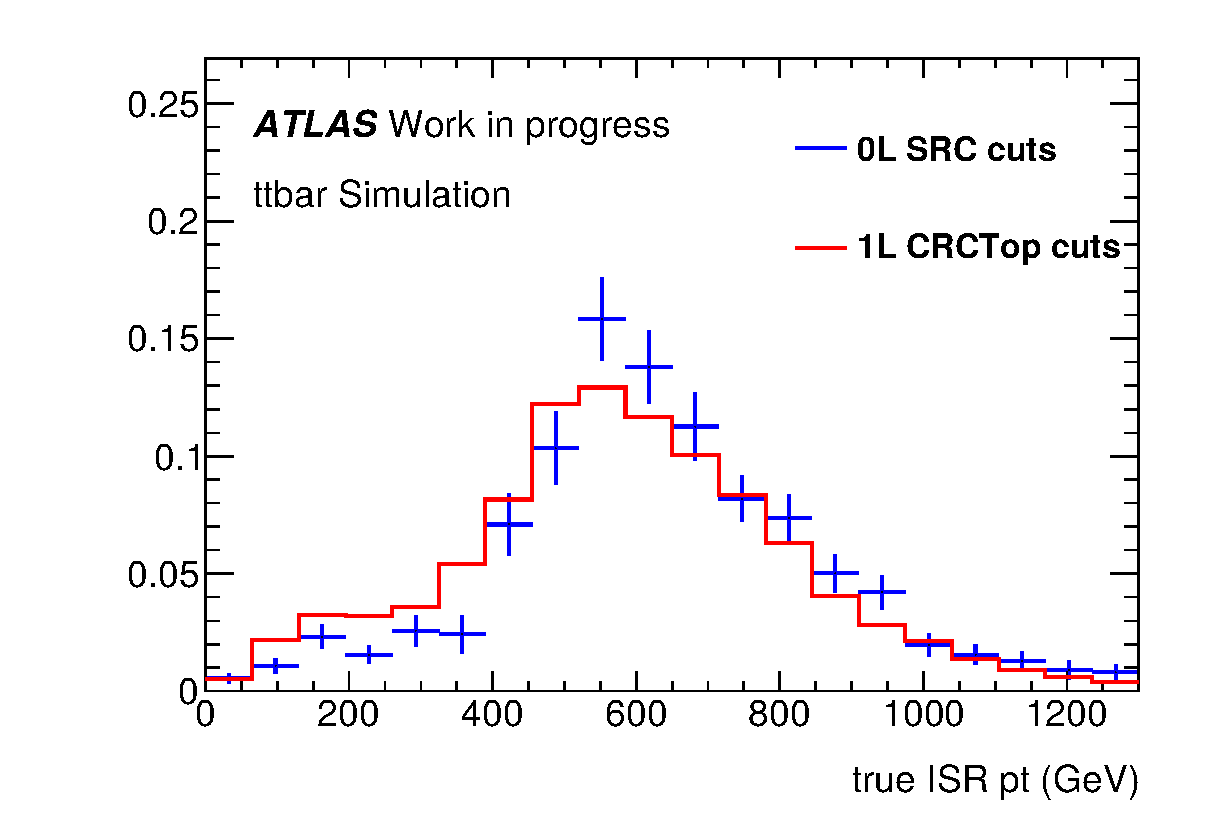
\includegraphics[width=0.65\textwidth]{./figures/ttbar/truePtISR_SRC_CRC_compare.eps}
%\caption{\label{fig:ttbar:CR:trueISRpt}{Distribution of true ISR pt for ttbar that survive the signal selections}}
%\end{figure}

%\indent In terms of branching fractions, the majority of ttbar branching fractions are to hadronic taus.  80 percent of the ttbar has one top decay via a single hadronic tau and the other top decays fully hadronically.  $15$ percent of the ttbar events decay via the single lepton channel where the lepton is an electron or a muon.  The lepton becomes lost because either it has too low pt to be reconstructed, removed because they were to close to another jet or is mis-reconstructed as a jet. The rest of the five percent composed of di-leptonic or lepton and tau ttbar events. Essentially no fully hadronic ttbar survives the zero lepton selection because fully hadronic ttbar do not make any hard neutrinos directly from the top decay.  \\
%\indent With such a large fraction of background coming from taus one might suspect setting up some sort of tau rejection.  However we found that a rejection based on loose tau IDs did not improve sensitivity.  The loss of signal was too large to justify the improvement in signal to background ratio.  The high jet multiplicity in signal gives a high probability of false positives.
%\indent Accepting mainly ttbar decay to hadronic taus gives a large boost signal to background due to branching fractions alone.  The two tops in signal events decay mainly through the fully hadronic channel.  Fully hadronic decays accounts for 44 percent of all ttbar decays.  On the other hand, the ttbar background mainly decay via hadronic taus which only accounts for about 10 of all ttbar decays.  We therefore gain a factor of 5 in signal to background ratio just by working in the zero lepton channel. This not only gains us a great boost in sensitivity in our SR.  It also allows us to design a ttbar control region with very similar selections to the SR but just in the single lepton channel.  We can avoid high signal contamination in our control region because both signal and background are mainly coming from single lepton decays in the 1 lepton channel.  As such, we no longer gain this factor of 5 in S/B based on branching fraction in the control region.  The details of the ttbar control region is described in section \ref{sec:Bkg:ttbar:CR} \\  

\subsection{Predicting the amount of $\ttbar$ in Signal Region using a One Lepton Control Region}
\label{sec:Bkg:ttbar:CR}

\indent Stop signal is expected to have a higher jet multiplicities and energy in the hemisphere containing $\met$ then both ttbar populations.  The stringent SR requirements on the jet multiplicities and total energy of the sparticle hemisphere effectively eliminate the top/anti-top back-to-back ttbar population and also rejects approximately $2/3$ of ttbar plus strong ISR population.  A detailed explanation of SR design and performance can be found in chapter \ref{chap:SignalRegion}. \\

\indent The ttbar events that survives the SR selections are composed of almost exclusively ttbar that are also produced with strong ISR.  Approximately 90 percent of the ttbar events in SR have an ISR pt of at least 400 $\gev$.  A back of the envelope calculation shows that we need around 550-600 $\gev$ of ISR $\pt$ to boost the ttbar neutrino to above 250 $\gev$ of $\pt$.  The neutrino must share the ISR $\pt$ with 5 other ttbar decay products and is not particularly efficient at absorbing ISR $\pt$.  Figure \ref{fig:ttbar:SR:trueISRpt} shows that the true ISR $\pt$ distribution for ttbar in SR peaks at approximately 550 $\gev$.  This demonstrates that the SR does indeed capture only ttbar with strong ISR $\pt$.  \\

\indent A direct consequence of selecting for only strong ISR ttbar is that the predicted ttbar background rates in SR is directly related to the amount of ISR/FSR in the MC.  The next-to-leading order (NLO) \textsc{Powheg+\pythia6} ttbar MC gives upwards of 30 percent uncertainty due to ISR/FSR systematic.  The ISR/FSR theoretical uncertainty would completely dominate if we relied on MC to predict SR ttbar rates.  \\

\indent In order to decrease the ISR/FSR uncertainty, we directly measure the ttbar plus strong ISR rate in data using an one lepton ttbar CR (CRCTop).  One lepton here refers only to electron and muons because they can be reconstructed with much greater purity then taus.  The selections used to define the CRCTop is defined in table \ref{tab:ttbar1LepCRISR_def}. All variables used are defined in section \ref{Jigsaw:Variables}. \\

\begin{table}[htpb]
  \caption{One-lepton \ttbar+ISR control region (CRCTop) definitions. The same \met\ triggers as mentions in Table~\ref{tab:SRcommon} are used. }
  \begin{center}
    \def\arraystretch{1.4}%
    \begin{tabular}{c|c} \hline\hline
      {\bf Variable}     & 1L 1b \ttbar CR \\ \hline \hline
      \multicolumn{2}{c}{1 Lepton Pre-Selection}  \\ \hline
      $N_{lep}$  & 1                   \\
      \mtlepmet          & $<80\gev$           \\ 
      \mindrblep         & $<2.0$              \\ 
      \NjV               & $\ge5$              \\
      \NbV               & $\ge1$              \\
      \pTSFour           & $>40\gev$           \\
      \PTISR             & $\ge 400$           \\ \hline \hline
    \end{tabular}
  \end{center}
  \label{tab:ttbar1LepCRISR_def}
\end{table}%

\indent CRCTop captures the same kinematic features as SR by targeting ttbar also produced with strong ISR $\pt$.  The CR uses similar selections on the same kinematic variables as SR.  The correlations on ISR and $\met$ are removed to increase statistics and lower signal contamination.  For example, $\dphiISRI$ specifies the direction of neutrino relative to the direction of the ISR.  A requirement of $\dphiISRI>3.0$ essentially selects specific ttbar decay axis.  Removing this cut opens up more phase space to ttbar decays but does not change the requirement on strong ISR $\pt$. \\

\indent Figure \ref{fig:ttbar:CR:trueISRpt} shows the true ISR $\pt$ distribution for ttbar in SR and CR.  Both distributions peak at roughly 550 $\gev$ and have similar shapes.  The one lepton CR essentially measures the amount of ttbar plus strong ISR directly in data.  By normalizing ttbar background rates to the CR, we are able to limit the ISR/FSR uncertainty to below 10 percent for all $\RISR$ regions.  \\

\indent The close kinematic selection between CRCTop and SR also allow leads to cancelation of other systematics.   For example, the 6 percent uncertainty on jet energy scale and jet energy resolution can be partial attributed to the CR and SR requiring jets of similar $\pt$. A more detailed discussion of systematics can be found in chapter \ref{chap:Uncertainties} \\

\begin{figure}[h!]
  \centering
	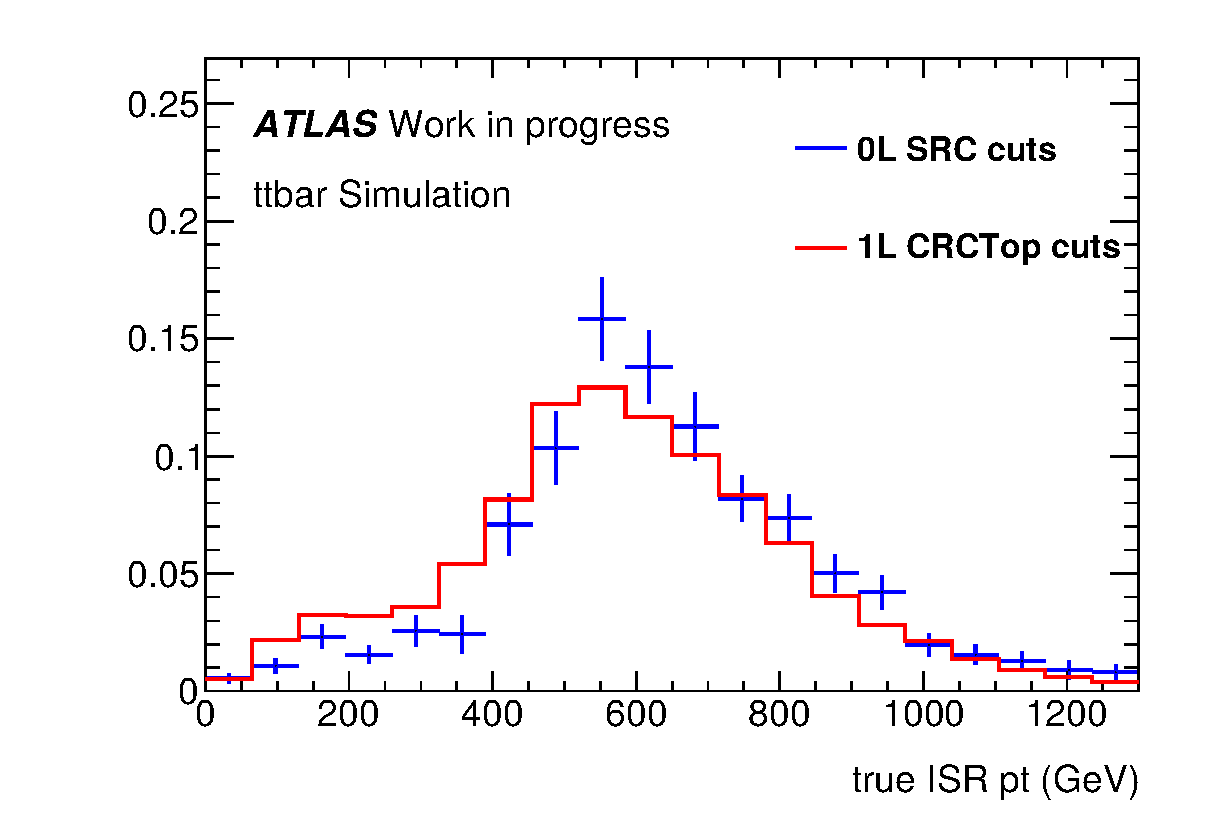
\includegraphics[width=0.65\textwidth]{./figures/ttbar/truePtISR_SRC_CRC_compare.eps}
\caption{\label{fig:ttbar:CR:trueISRpt}{Distribution of true ISR pt for ttbar that survive the CR and SR selections.  Both peak at roughly 550 $\gev$ demonstrating that the one lepton CR and zero lepton SR captures the same population of ttbar plus strong ISR.  Therefore, the one lepton CR essentially measures the amount of ttbar in SR directly from data with little extrapolation over ISR $\pt$.}}
\end{figure}

\indent In the one lepton CRCTop, the lepton is included as a ``jet'' in the Jigsaw ISR algorithm and will be counted as a sparticle jet or an ISR jet depending on which hemisphere it falls.  The lepton is meant to play the role of a hadronic tau jet in the zero lepton SR.  This approximation is justified since roughly 80 percent of all ttbar events in SR decay via the hadronic tau channel.  \\

\indent  Stop signal, especially those with $\Delta m \neq m_{t}$, tend to produce more $\met$ because of the presence of neutralinos.  A cut of $\mtlepmet < 80\gev$ is added to remove signal contamination.  
A $\mindrblep<2.0$ cut is added to increase ttbar purity and ensure orthogonality to the W+jets control region. \\

\indent The $\pTjV>50\gev$ cut is relaxed to $\pTjV>40\gev$ in order to increase statistics in the CR.  The $\pTjV$ cut specifies the $\pt$ of the 4th jet in the sparticle system.  The $\pTjV$ cut can be correlated with ISR/FSR because there is a chance that the 4th most energetic jet in the sparticle system is from radiation and not from a top decay.  However for this analysis it is more important to accurately gauge the amount of hard ISR of order hundred or more GeV that the ttbar system recoils against then amount of additional radiation in the same hemisphere as $\ttbar$. We found that loosening $\pTjV$ cut to 40 GeV does not result in a large difference in the true ISR pt distribution in the CRCTop and SR. \\

\subsubsection*{CRCTop Signal Contamination}

\indent Signal contamination in CRCTop ranges from 1 percent at high stop masses to 12 percent at low stop masses for all mass points not already excluded by previous stop experiments.  The largest signal contamination occurs at a stop mass of 225 to 250 $\gev$.   Here, the signal contamination approaches 12 percent due to the large stop production cross-section.  Lower stop masses result in higher signal contamination but our search does not have sensitivity to regions below 225 $\gev$.  \\

\indent The fact that CRCTop can attain such low signal contamination while selecting for ttbar background with such similar kinematic features as SR is impressive.  The SR has a signal to background ratio of approximately 2 to 1 for stop masses between 250 $\gev$ and 400 $\gev$.   In comparison, CRCTop is able to achieve SR contamination of around 5 to 12 percent for the same signal points.  \\

\indent CRCTop is able to make up for this factor of 20-40 difference in S/B rate mainly due to two reasons.  First CRCTop is a one lepton control region.  Working in the one lepton region means both signal and ttbar background draw from the single muon and single electron decay channels.  Signal and background therefore has similar decay fractions in CRCTop. The SR, on the other hand, mainly selects for signal with two tops that decay fully hadronically with roughly a 44 percent branching fraction.  In comparison, the ttbar background in SR main decay via the single hadronic tau decay channel with only a 10 percent decay fraction.  The CR therefore has a factor of 5 decrease in S/B ratio compared to the SR based on branching fraction alone.  \\

\indent The SR also gains S/B by enforcing the correlations between the ISR system and $\met$.  Removing the $\dphiISRI > 3.0$ requirements decreases S/B by another factor of 3. Including all regions of $\RISR$ in CRCTop and specifically targeting the $\RISR$ window under the signal peak decreases the S/B of 2 to 5 to the S/B depending on the stop mass and location of signal $\RISR$ peak.  Removing the requirement on these correlations do no change the requirement on strong ttbar ISR $\pt$ but opens up more phase space for ttbar to decay.  \\

\indent The two factors combine to make up the roughly factor of 30 decrease in S/B between SR and CRCTop; all the while preserving the agreement in true ttbar ISR $\pt$ distribution shown in figure \ref{fig:ttbar:CR:trueISRpt}. \\

\subsubsection*{CRCTop Distributions}

\indent Distribution of important variables after normalization to $\intlumi$ $\ifb$ of data are shown for CRCTop in figure \ref{fig:CRTopC}.  There seem to be no significant slope in the data over MC comparison in the CRCTop $\pTjV$ distribution.  This is further evidence that the extrapolation from 40 to 50 GeV across $\pTjV$ is allowed.  \\

\indent There is a noticeable trend in the data over MC comparison in the CRCTop $\pTISR$ distribution.  The disagreement is not surprising given that a priori we have an 30 percent uncertainty due to the ISR/FSR uncertainty.  This further demonstrate the need for a CR that directly measures the amount of ttbar with strong ISR pt in data. \\

\begin{figure}[htbp]
  \begin{center}
    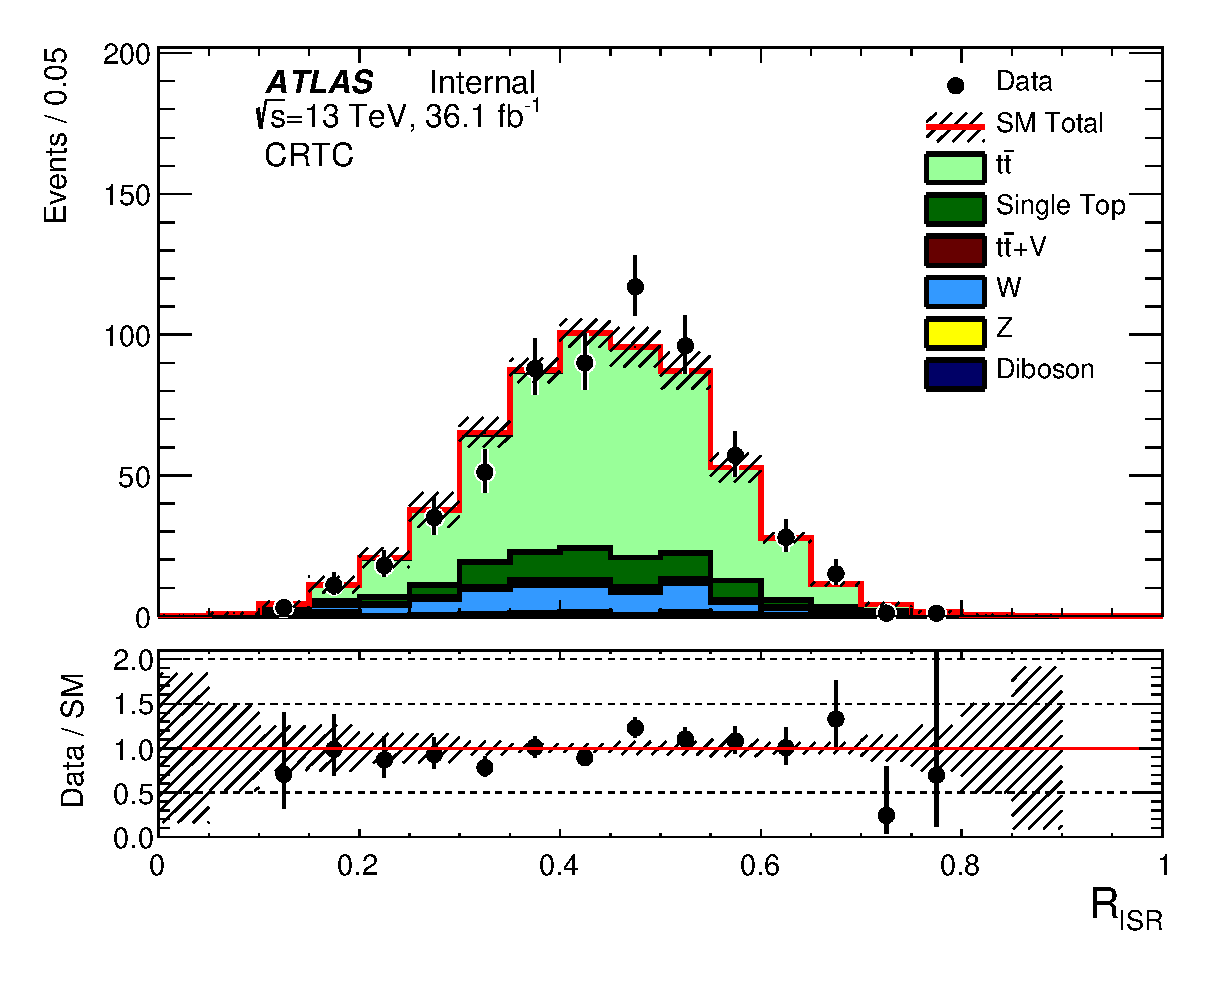
\includegraphics[width=0.45\textwidth]{figures/ttbar/postfit/CA_RISR_CRTopC}
    \includegraphics[width=0.45\textwidth]{figures/ttbar/postfit/CA_pTISR_CRTopC}
    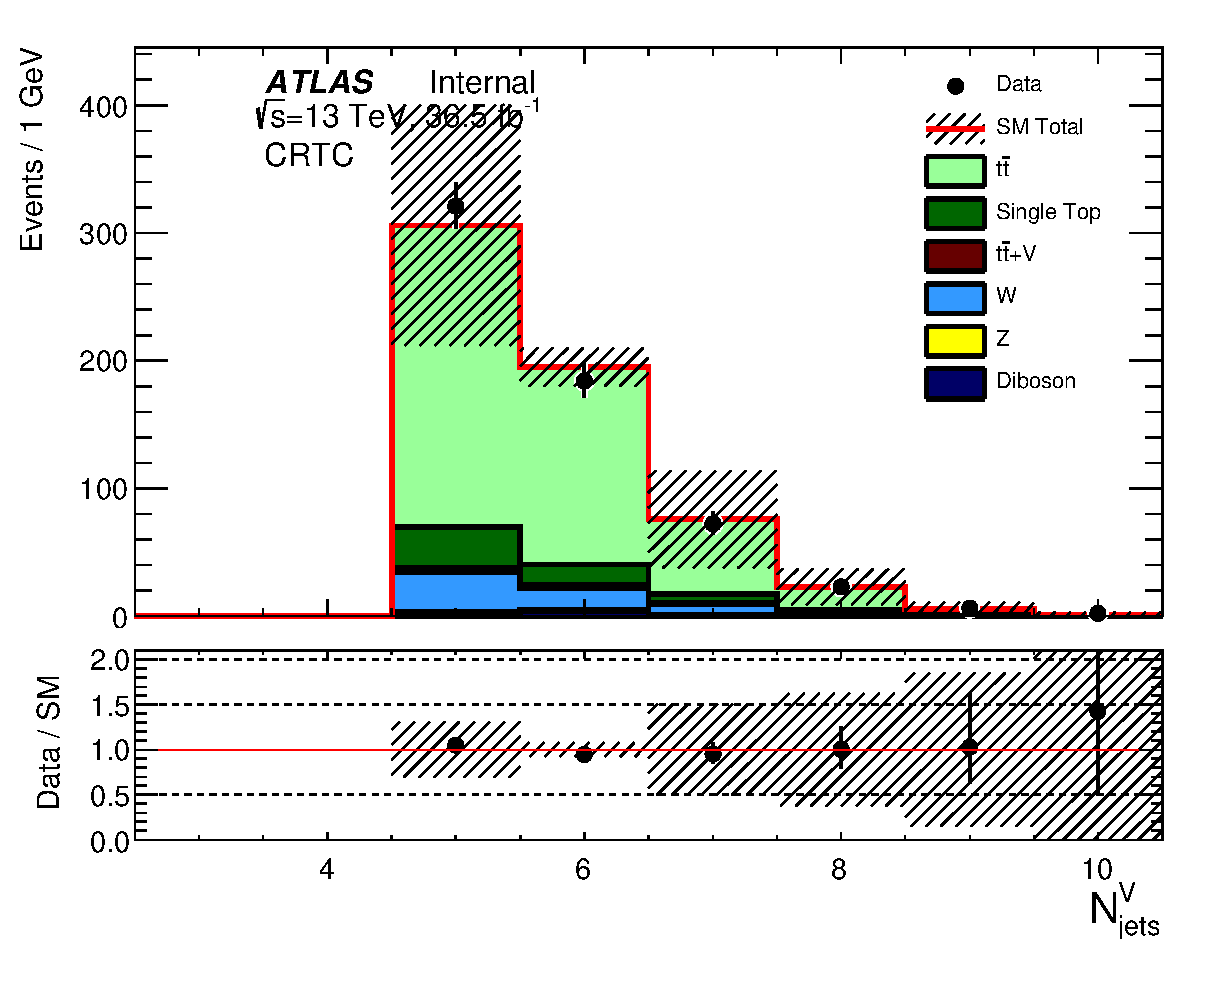
\includegraphics[width=0.45\textwidth]{figures/ttbar/postfit/CA_NjV_CRTopC}
    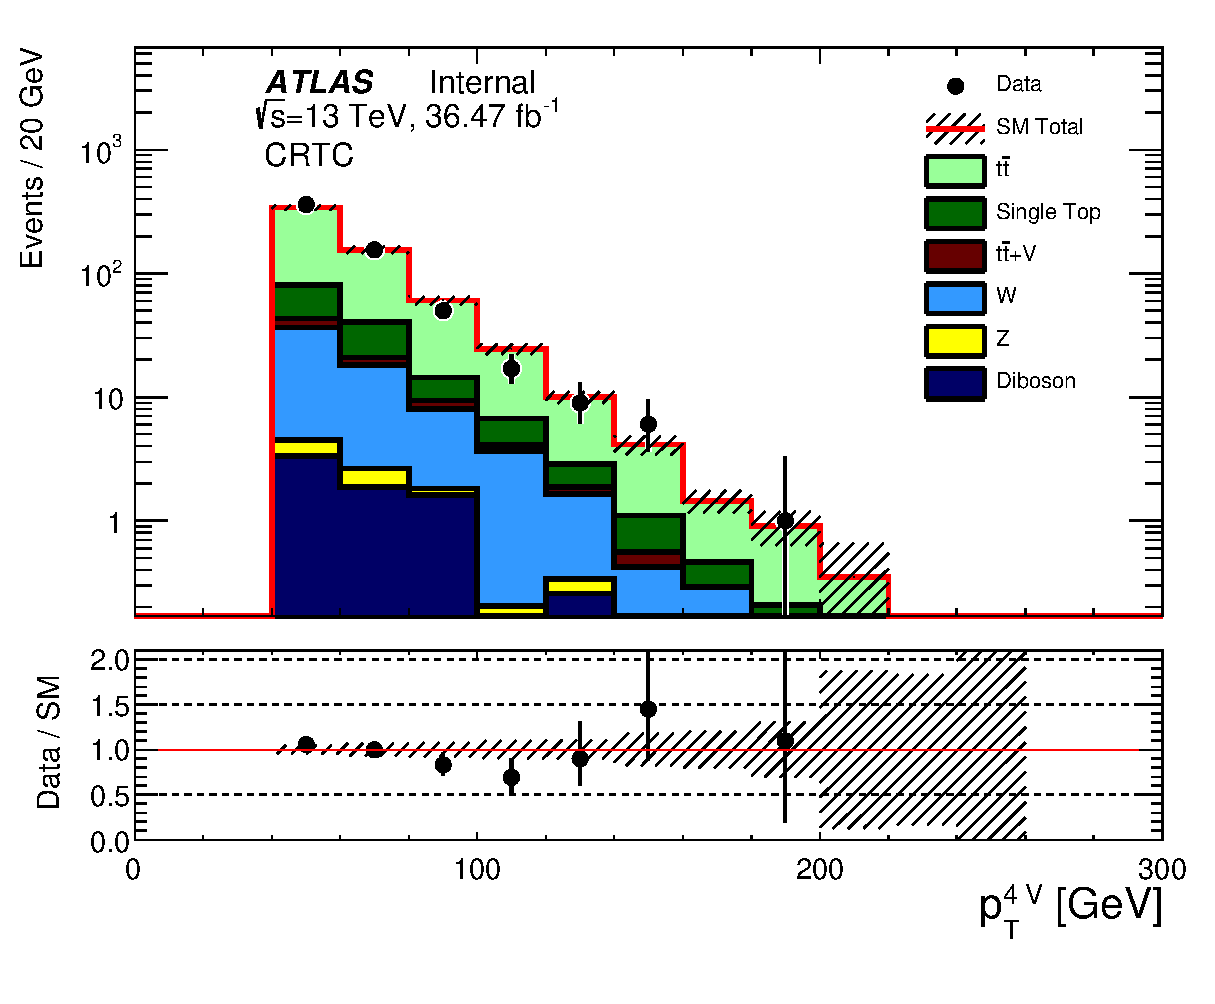
\includegraphics[width=0.45\textwidth]{figures/ttbar/postfit/CA_pTjV4_CRTopC_log}
    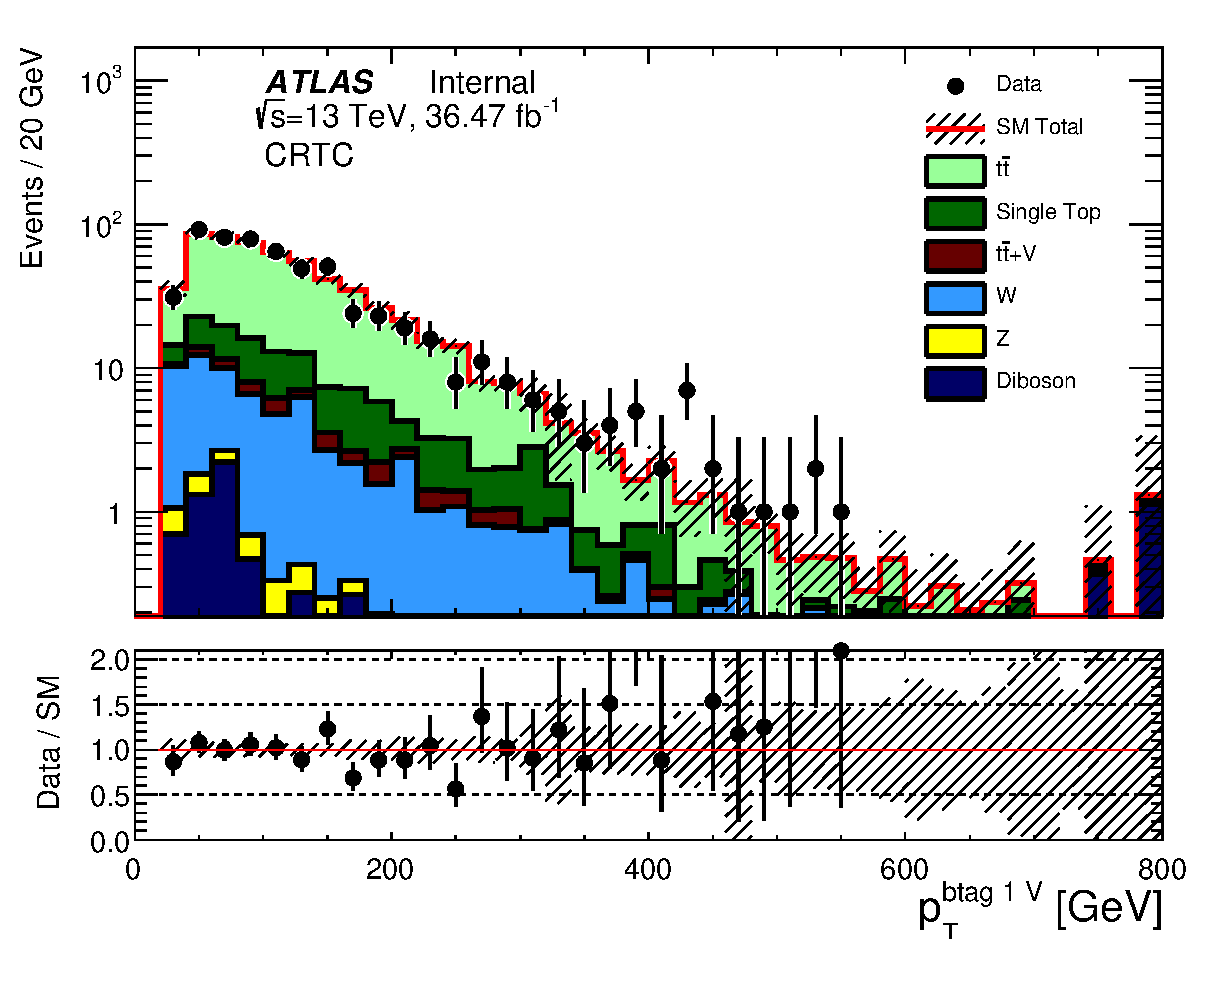
\includegraphics[width=0.45\textwidth]{figures/ttbar/postfit/CA_pTbV1_CRTopC_log}
        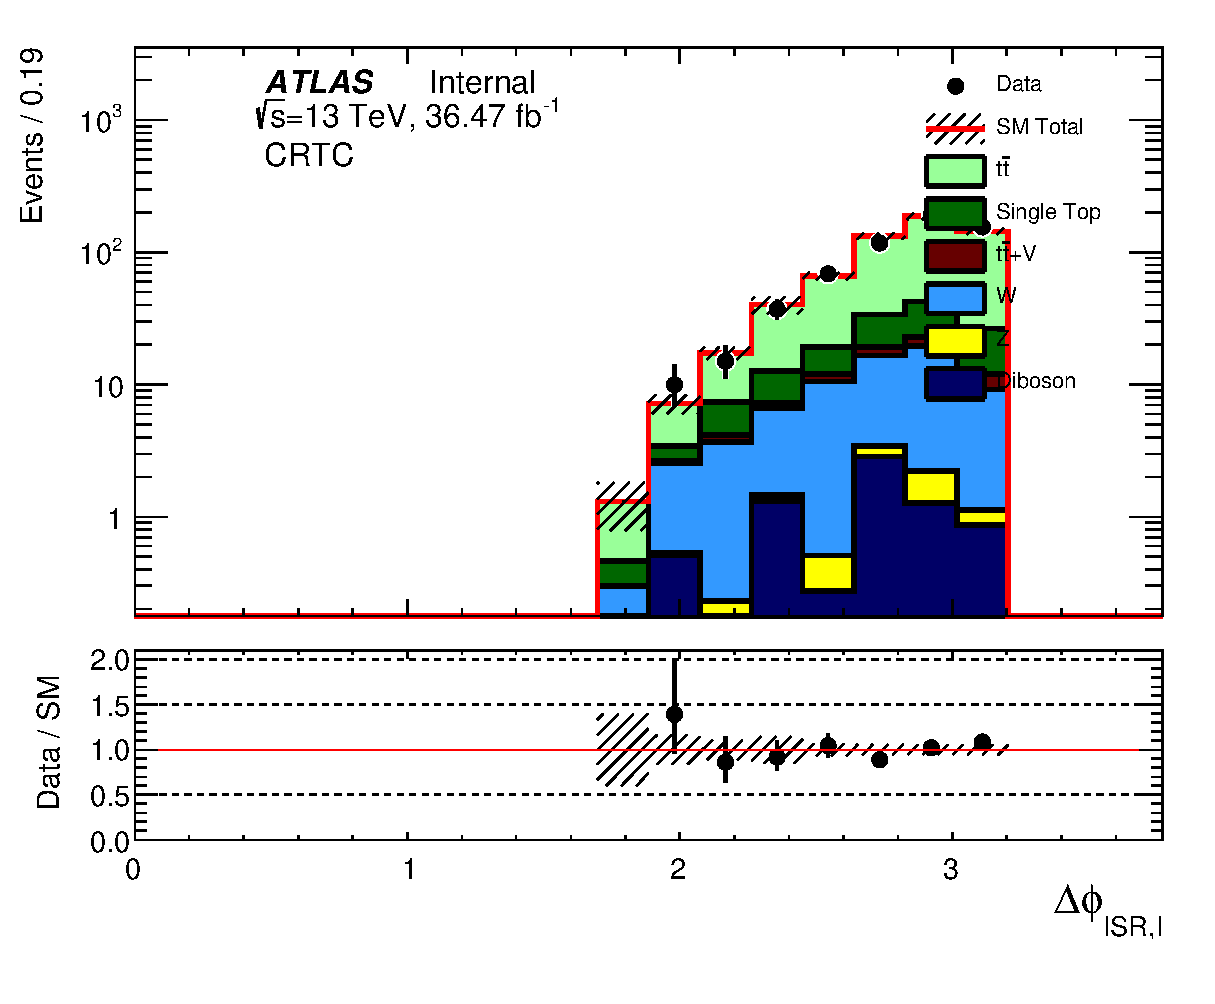
\includegraphics[width=0.45\textwidth]{figures/ttbar/postfit/CA_dphiISRI_CRTopC_log}
  \end{center}
  \caption{One lepton ttbar CR (CRCTop) distributions for $\intlumi$ $\ifb$ of data. All backgrounds have already been normalized to CRs by performing a background only fit.  The ratio between data and MC is shown in the bottom panel. The hashed area in both the top and lower panel represent the uncertainty due to MC statistics and detector systematic uncertainties.}
  \label{fig:CRTopC}
\end{figure}

\indent The normalization scale factor for ttbar is 0.707 according to a background only fit on $\intlumi$ $\ifb$ of data. This scale factor is quiet different from 1.0 which indicates that the ttbar MC alone does not well model the high ISR $\pt$ phase space.  Again, this difference is not unexpected given the 30 percent ISR/FSR uncertainty on ttbar MC.  \\

\subsection{Validating $\ttbar$ Predictions in Signal Region using a Zero Lepton Validation Region}
\label{sec:Bkg:ttbar:VR}

\indent We also define a zero lepton ttbar VR to validate the predicted background rates in SR.  The ttbar VR (VRCTop) is kinematically similar to SR but has the $\dphiISRI < 3.0$ selection is inverted to ensure orthogonality and limit signal contamination. In ttbar events, $\dphiISRI$ specifies the direction of neutrino relative to the direction of the ISR.  Inverting the $\dphiISRI$ selection only selects for ttbar with a different decay axis but does not change the requirements on strong ISR $\pt$.  The $\dphiISRI < 3.0$ selection does effectively reject stop events because the neutralinos gain all their momenta from the ISR system in signal. \\

\indent The requirement on $\MS$ is reduced to 100 GeV (vs. 300 GeV in the SR) and an $\NjV \ge 4$ selection is applied (vs. $\NjV \ge 5$ in the SR) to enhance the yields of semi-leptonic $\ttbar$ events . A requirement of $\MV/\MS < 0.6$ is added to reduce signal contamination and reject QCD multijet background. \\

\indent Similar to CRCTop, the $\pTjV>50\gev$ selection is relaxed to $\pTjV>40\gev$ to increase VR statistics. \\

\begin{table}
  \caption{Zero-lepton \ttbar+ISR validation region definitions, in addition
    to the SRC requirements listed in Table~\ref{tab:SRcommon}.}
  \begin{center}
    \def\arraystretch{1.4}%
    \begin{tabular}{c||c} \hline\hline
      {\bf Variable} & \\ \hline \hline
      \NjV           & $\ge4$                \\
      \NbV           & $\ge1$                \\
      \pTbV          & $\ge 40$              \\
      \PTISR         & $\ge 400$             \\
      \MS            & $>100\gev$            \\
      $\MV/\MS$      & $<0.6$                \\
      \dphiISRI      & $<3.00$               \\ \hline \hline
    \end{tabular}
  \end{center}
  \label{tab:ttbar0LepVR}
\end{table}%

\indent The distributions of the selection variables in VRCTop are shown in Fig.~\ref{fig:ttbar0Lep1bVRISR}.  The background rates have been normalized to CRs through the use of a background only fit to $\intlumi$ $\ifb$ of data. \\

\begin{figure}[htbp]
  \centering
    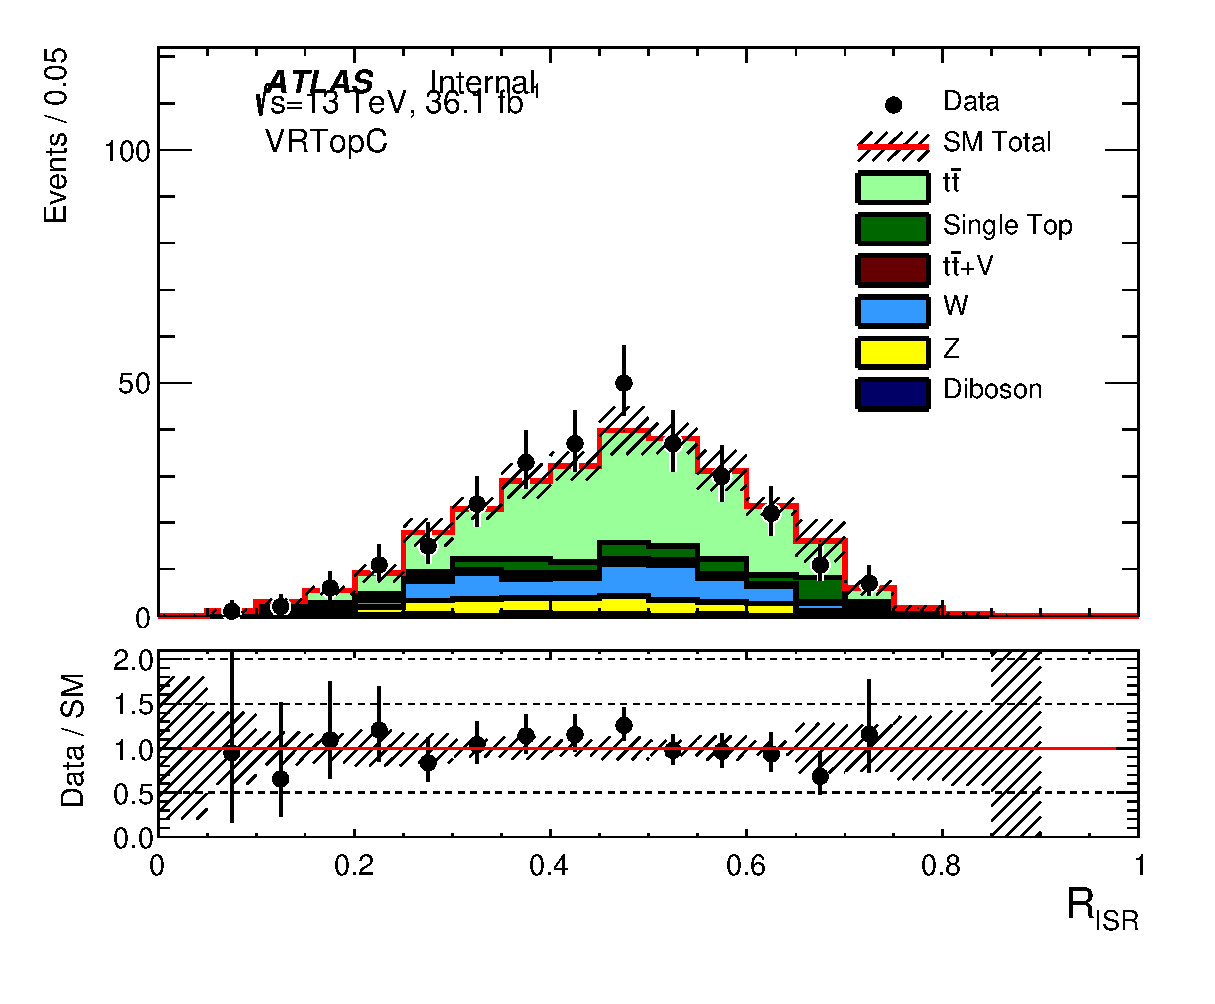
\includegraphics[width=0.45\textwidth]{figures/ttbar/postfit/CA_RISR_VRTopC}
    \includegraphics[width=0.45\textwidth]{figures/ttbar/postfit/CA_pTISR_VRTopC}
    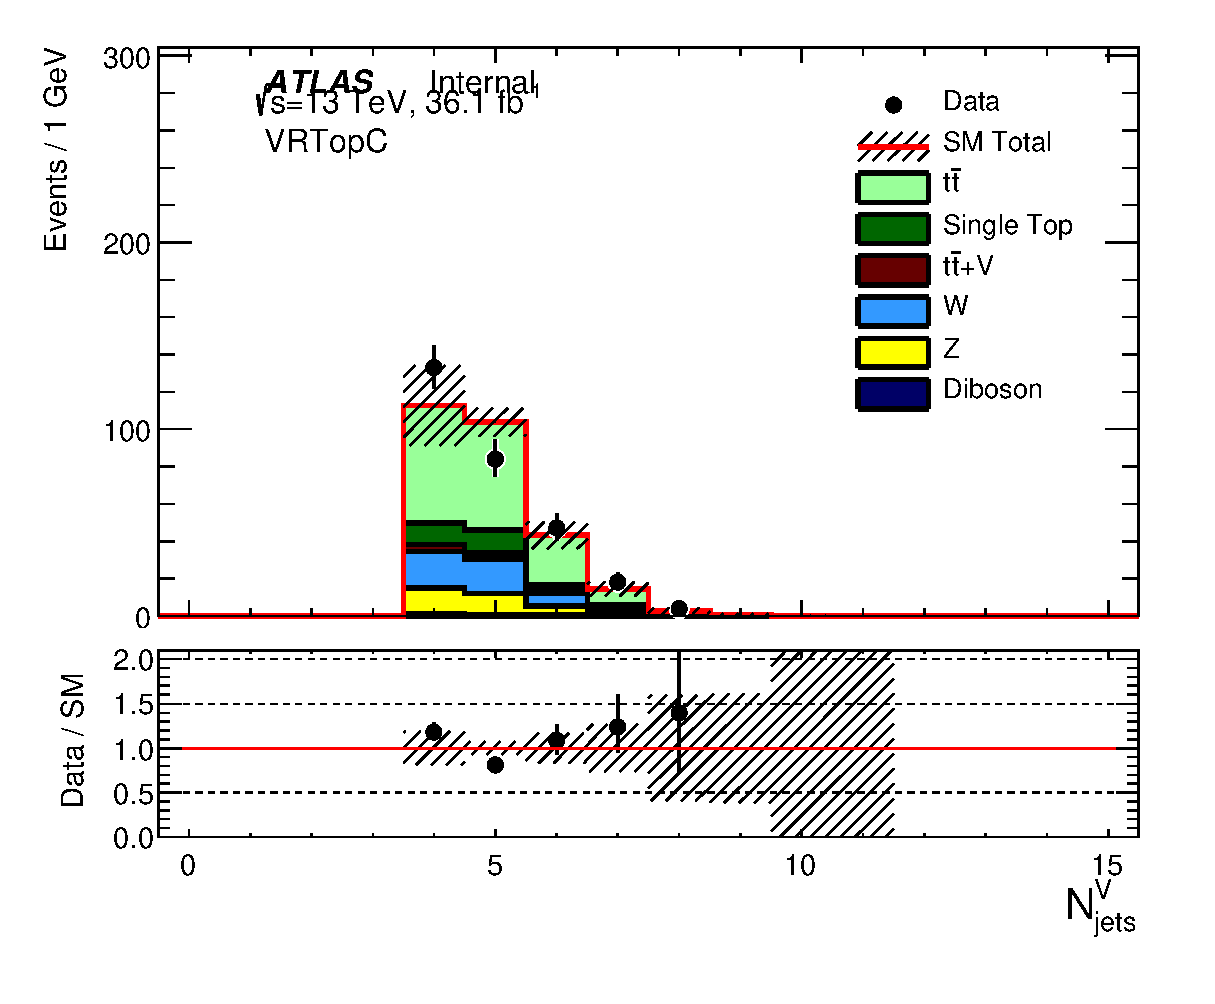
\includegraphics[width=0.45\textwidth]{figures/ttbar/postfit/CA_NjV_VRTopC}
    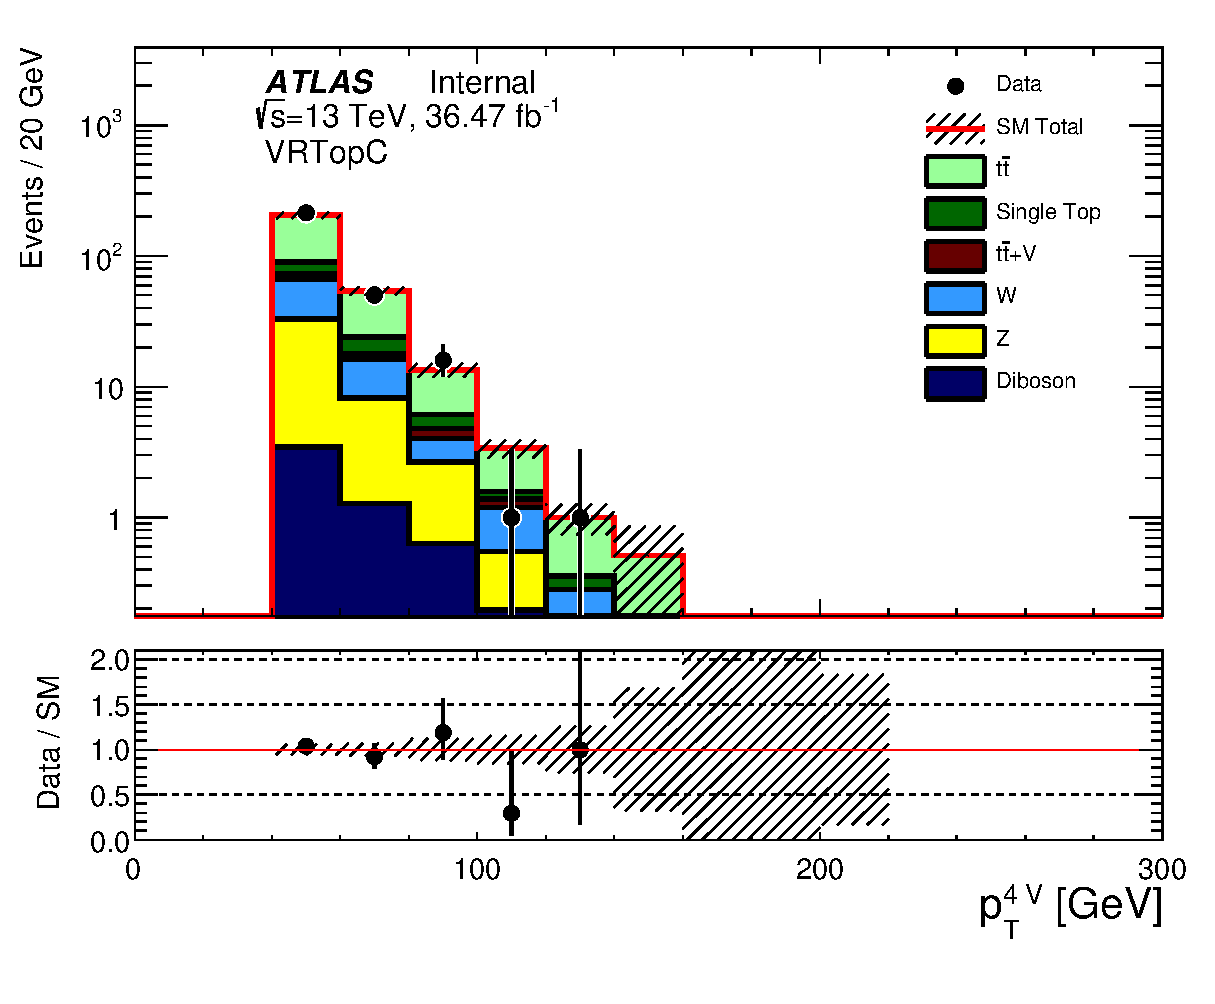
\includegraphics[width=0.45\textwidth]{figures/ttbar/postfit/CA_pTjV4_VRTopC_log}
    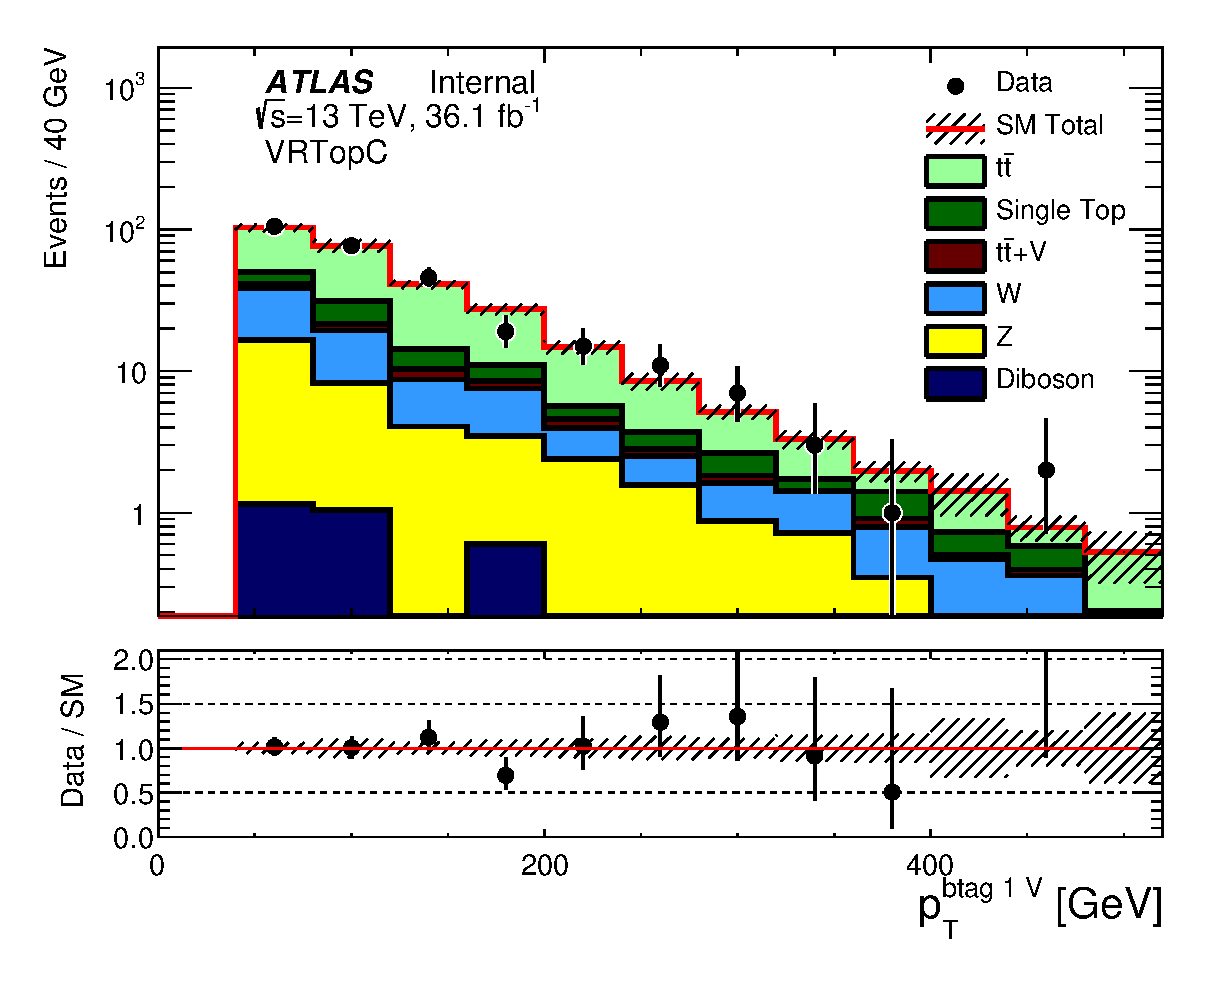
\includegraphics[width=0.45\textwidth]{figures/ttbar/postfit/CA_pTbV1_VRTopC_log}
        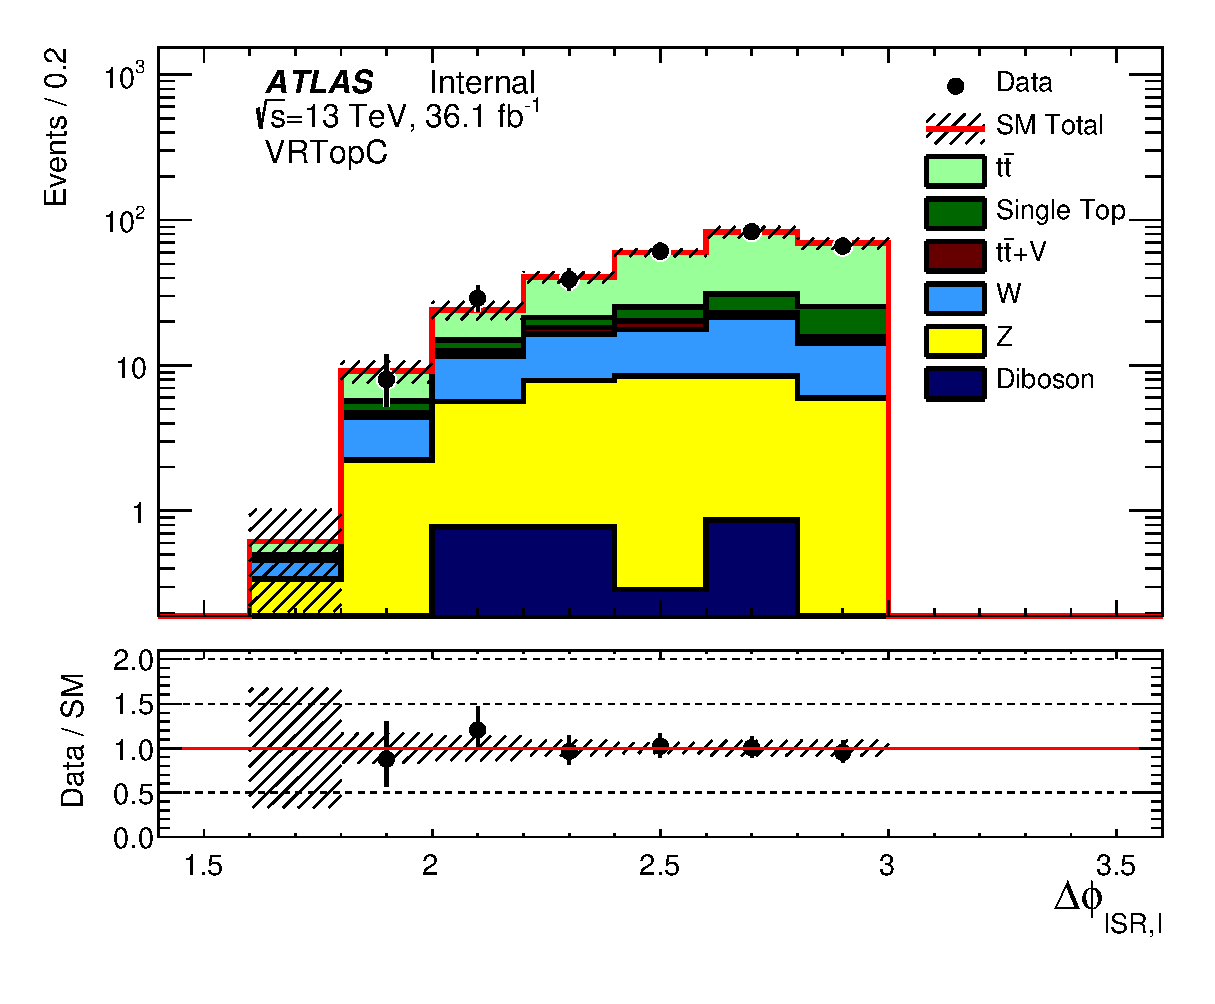
\includegraphics[width=0.45\textwidth]{figures/ttbar/postfit/CA_dphiISRI_VRTopC_log}
  \caption{\label{fig:ttbar0Lep1bVRISR}{Distribution of select variables in the zero lepton ttbar validation region.  The ratio between data and MC predictions are shown in the bottom panel.  The background rates have been normalized to CRs through the use of a background only fit to $\intlumi$ $\ifb$ of data.  Experimental systematic uncertainties on background predictions are depicted as the hashed bands. }}
\end{figure}

\indent The predicted background rate in the VRCTop agrees with data to within $1\sigma$.  This demonstrates that CRCTop is an effective predictor of ttbar background rates in VR and SR.  The $\RISR$ shape is well modeled as we see no distinct trends in the data vs MC ratio in $\RISR$. \\

\indent Similar to CRCTop, there is a noticeable trend in the data over MC comparison in the VRCTop $\pTISR$ distribution.  Again this is expected because the MC is a poor predictor of ISR $\pt$ rates.  The fact that data in VRCTop agrees with the predicted background rate proves that CRCTop can effectively measure the amount of ttbar with at least 400 $\gev$ of ISR $\pt$.  \\

%\indent This agreement both in magnitude and shape demonstrates two things.  One, the ttbar control region indeed does correctly measure the amount of ttbar plus strong ISR that exists in both signal and validation region.  Two, the sub-dominant background predictions also cannot by wrong by more than around 100 percent.  For example we clearly would see disagreement in between data vs MC in this VR if the MC underestimated W+jets or Z+jets background by 100 percent.  Both of these facts gives us confidence that the predictions for the amount of background in the SR is correct. \\